\documentclass[aspectratio=169, 14pt,usenames,dvipsnames]{beamer}
\usetheme{TalentSprint}
\usepackage[utf8]{inputenc}
\usepackage{graphics}
\usepackage{ragged2e}
\usepackage{amsfonts}
\usepackage{xcolor}
\usepackage{tcolorbox}
\usepackage{setspace}


\definecolor{swe}{rgb}{0.19, 0.73, 0.56}

\usepackage{verbatim}
\usepackage{csquotes}
\title[Linear Classifier]{Linear Classifier}


\begin{document}

{\1
\begin{frame} 
%	\title[Linear Classifier]{Linear Classifier}
	\subtitle{Classification Algorithms}
	\maketitle
\end{frame}
}

\begin{frame}{What is Linear?}
\begin{columns}
\column{0.5\textwidth}
\begin{itemize}
\item  Recall the abstraction:
\begin{itemize}
\item  $ \alert{y=f(w,x)}$
\end{itemize}
\item  If \alert{f} is linear, we have a Linear Classifier
\textcolor{red}{\item $ f = \Sigma w_ix_i = W^T{\cdot}X $}
\end{itemize}
\column{0.5\textwidth}
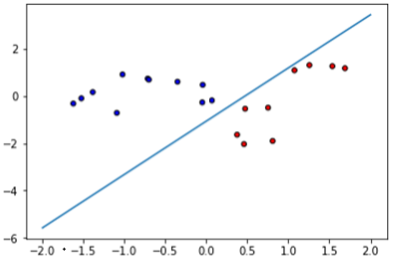
\includegraphics[width=6cm,height=4cm]{Images/2lcla.png}
\end{columns}
\end{frame}



\begin{frame}{Linear Classifier}
\begin{columns}
\column{0.5\textwidth}
\begin{itemize}
	\item  If \alert{$ W^T{\cdot}X \geq 0$} then Class 1 \vspace {5pt}
	\item  If \alert{$ W^T{\cdot}X \textless 0$} then Class 0
\end{itemize}
\column{0.5\textwidth}
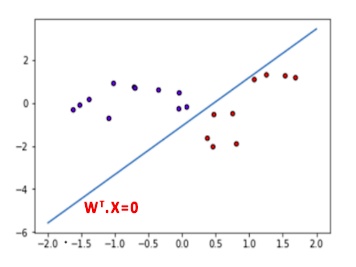
\includegraphics[width=6cm,height=4.5cm]{Images/3lcla.png}
\end{columns}
\end{frame}


\begin{frame}{Linear Classifier}
\begin{columns}
\column{0.5\textwidth}
	\textbf{\alert{Data:}}
\begin{itemize}
\item Apples (red)
\item Oranges (green)
\item Test: Unknown (blank)
\end{itemize} 
\textbf{\alert{Goal}}
\begin{itemize}
\item Find a line that separates
\end{itemize}

\column{0.5\textwidth}
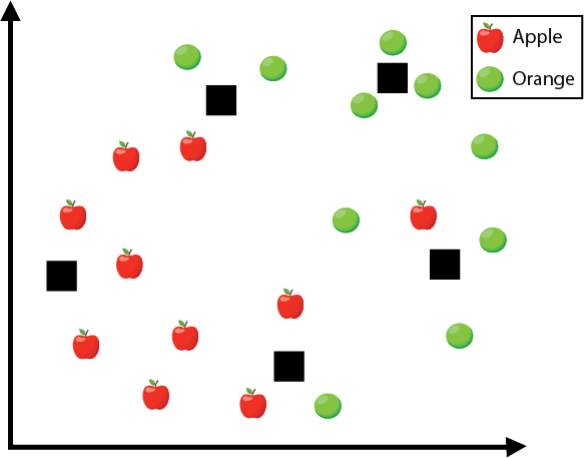
\includegraphics[width=7cm,height=5cm]{Images/4lcla.png}
\end{columns}
\end{frame}



\begin{frame}{One Solution: $x_1 + 2x_2 + 2 = 0$}
\begin{columns}
\column{0.5\textwidth}
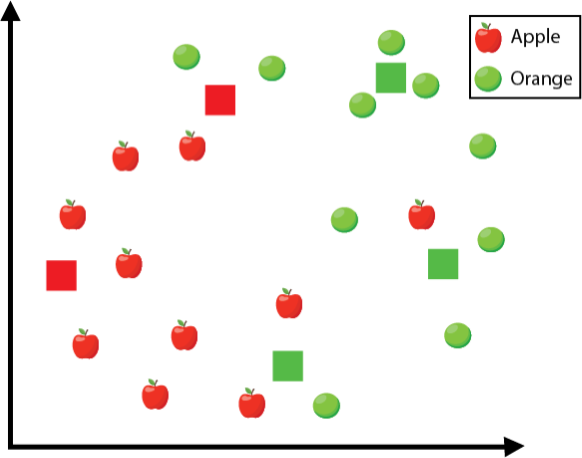
\includegraphics[width=7cm,height=5cm]{Images/5lcla.png}
\column{0.5\textwidth}
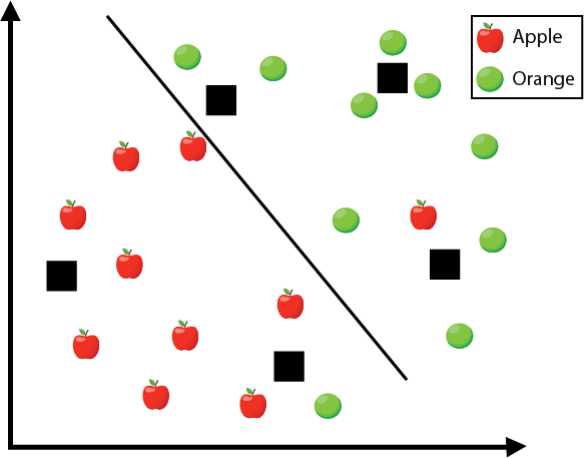
\includegraphics[width=7cm,height=5cm]{Images/5alcla.png}
\end{columns}
\end{frame}


\begin{frame}{What is the Error/Accuracy?}
\begin{columns}
\column{0.45\textwidth}\\
	\centering On the test data: \\ \centering 40\% error \\[8pt]
On the training data: \\ \centering 10\% error
\column{0.5\textwidth}
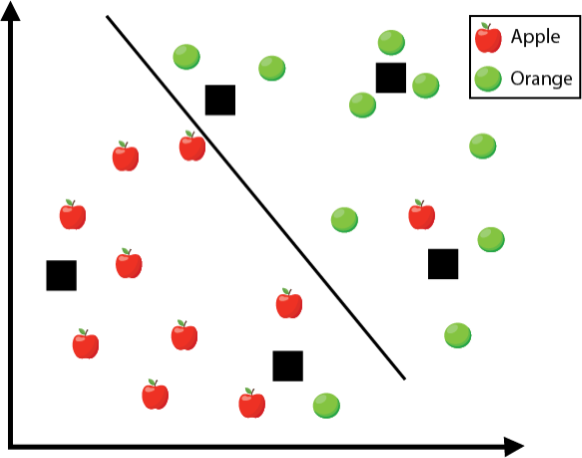
\includegraphics[width=8cm,height=5.5cm]{Images/6lcla.png}
	\column{0.05\textwidth}
\end{columns}
\end{frame}


\begin{frame}{Best Solution: $2x_1 - 4x_2 - 5 = 0$}
\begin{columns}
\column{0.5\textwidth}
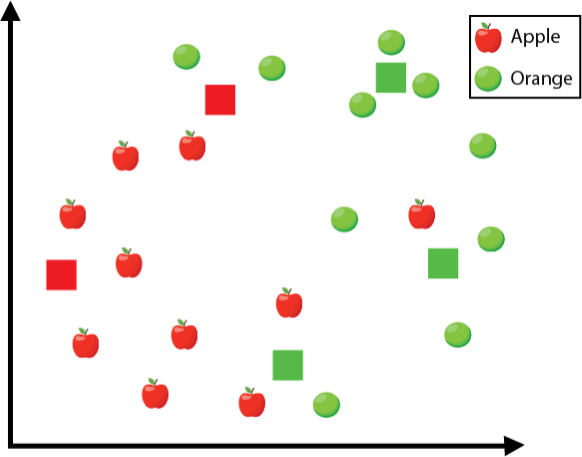
\includegraphics[width=7cm,height=5.5cm]{Images/7lcla.png}
\column{0.5\textwidth}
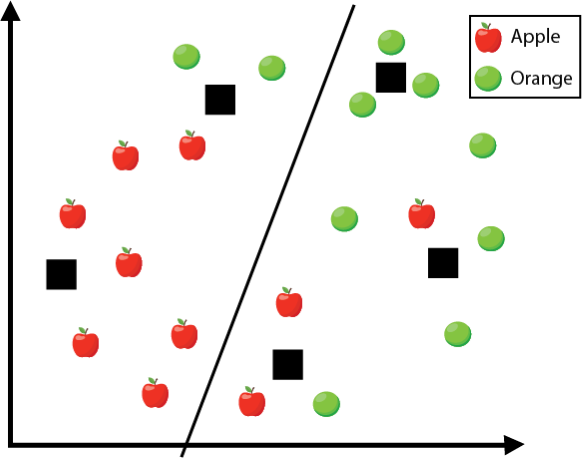
\includegraphics[width=7cm,height=5.5cm]{Images/7alcla.png}
\end{columns}
\end{frame}



\begin{frame}{What is the Error/Accuracy?}
\begin{columns}
\column{0.45\textwidth}\\
	\centering On the test data: \\ \centering 0\% error \\[8pt]
On the training data: \\ \centering 25\% error
\column{0.5\textwidth}
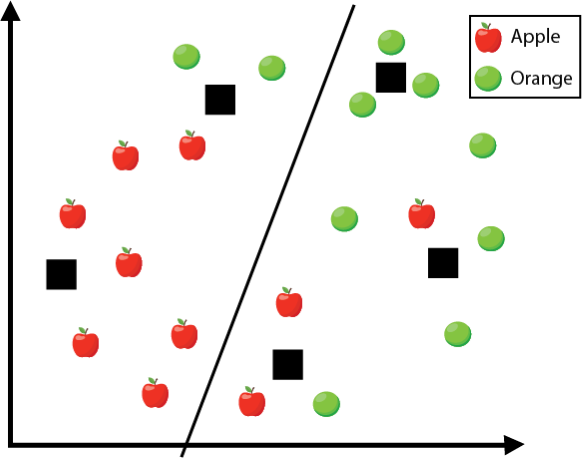
\includegraphics[width=7cm,height=5.5cm]{Images/8lcla.png}
	\column{0.05\textwidth}
\end{columns}
\end{frame}




\begin{frame}{What is the “Learning” Problem?}
\begin{columns}
	\column{0.05\textwidth} \\
\column{0.45\textwidth}\\
Find the best line given \\ (only) the training \vspace{12pt}{data}

 
Find \alert{$\omega_1, \omega_2, \omega_0$} in \\ \alert{$\omega_1x_1 + \omega_2x_2 +\omega_0 = 0$}
\column{0.5\textwidth}
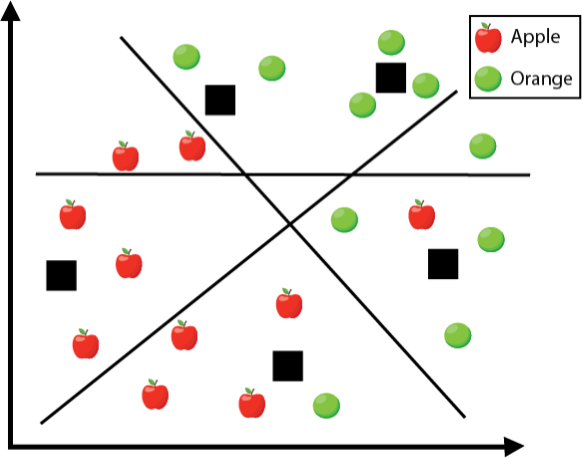
\includegraphics[width=7cm,height=5.5cm]{Images/10lcla.png}
\end{columns}
\end{frame}



\begin{frame}{Characteristics}

	\begin{itemize}
		\item \alert{Linear Classifier:}
			\begin{itemize}
				\item \alert{(d-1)} additions; \alert{d} multiplications
			\end{itemize}
		\item Simple at test  time.
		\item Additional \enquote{offline} training to find w
	\end{itemize}

	\hspace{6cm} \textcolor{blue}{N: Total number of samples \\ \hspace{6cm}  d: Total number of features \\ \hspace{6cm} or dimensionality}
\end{frame}

\begin{frame}{Understanding Linear Classifier as ``Neuron"}
\centering
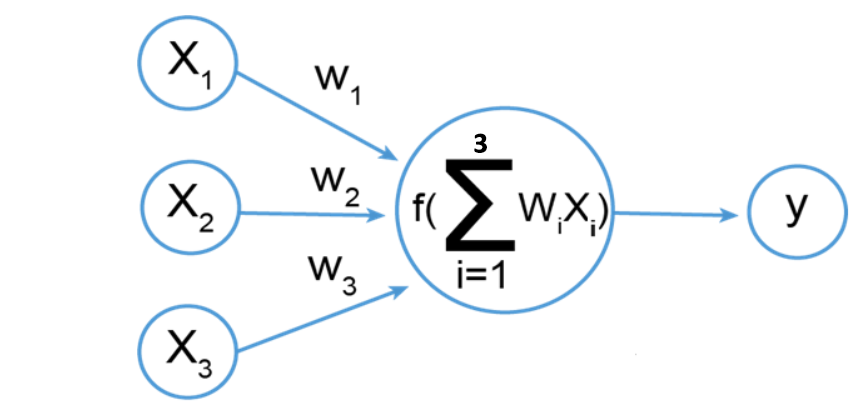
\includegraphics[width=0.9\textwidth, height=0.7\textheight]{Images/13lcla.png}
\end{frame}

\begin{frame}{Neural Networks}
\begin{columns}
\column{0.5\textwidth}
\begin{itemize}
\item Biologically inspired networks.
\item Complex function approximation through composition of functions.
\item Can learn arbitrary Nonlinear decision boundary
\end{itemize} 
\column{0.5\textwidth}
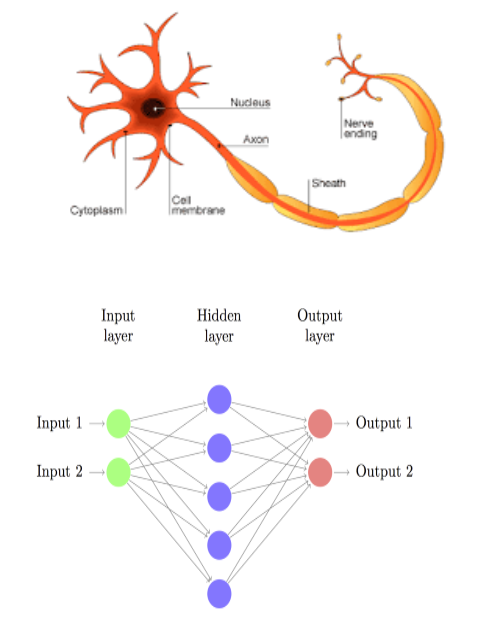
\includegraphics[width=5.2cm,height=5.75cm]{Images/14lcla.png}
\end{columns}
\end{frame}

\begin{frame}{A Peep into Deep Neural Networks}
\centering
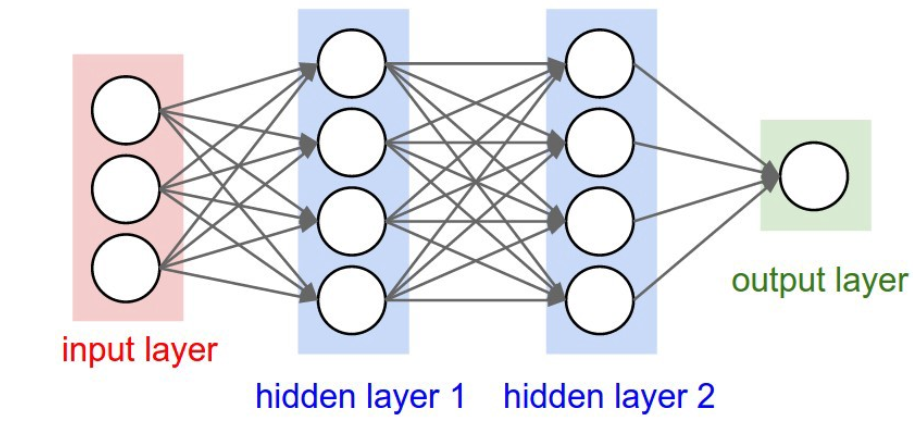
\includegraphics[width=0.8\textwidth, height=0.6\textheight]{Images/15lcla.png}
\end{frame}



\begin{frame}{Experiment}
\begin{itemize}
\item {Demo\_LC\_Penguins\_data} 
	\begin{itemize}
		\item Dataset : Penguins data 
		\item Objective : To apply Linear classifier to a multi-class classification problem
	\end{itemize}
\end{itemize}
\end{frame}



{\1   
\begin{frame}
\title{Thanks!!}
	\subtitle{Questions?}
	\titlepage
\end{frame}
}


\end{document}




